%	LaTeX template for the Collaborative Research Center proposal (3rd funding period) Oxyflame.
%	WSA, RWTH Aachen, 2020, (contact person: Stefan Pielsticker)

%%%% PLEASE ADJUST:
%\WorkInstruction{ Enter the number of the project here. Replace only the text "Example project" Please make sure that the project name corresponds exactly to the name of the folder of your project.}
% Example: \renewcommand{\Project}{A1}

\renewcommand{\Project}{Ex}
\renewcommand{\ChapterTitle}{Modeling solid fuel ignition, combustion and pollutant emissions}
\renewcommand{\ProjectTitle}{Direct numerical simulation and modelling of oxy-fuel combustion processes}



%%%% DON'T CHANGE ANYTHING FROM HERE UNTIL NEXT MARKER!
\chapter{\ChapterTitle}
%%%% DONT CHANGE ANYTHING UNTIL HERE!

%%%% PLEASE ADJUST:
\chapterauthor[1]{Pooria Farmand}
\chapterauthor[1]{Heinz Pitsch}


%%%% DON'T CHANGE ANYTHING FROM HERE UNTIL NEXT MARKER!
\begin{affils}
	%%%% DONT CHANGE ANYTHING UNTIL HERE!
	
	%%%% PLEASE ADJUST:
	\chapteraffil[1]{\RWTHITV}
	%\chapteraffil[2]{\RWTHITV}
	%\chapteraffil[3]{\RWTHAIA}
	
%%%% DON'T CHANGE ANYTHING FROM HERE UNTIL NEXT MARKER!
\end{affils}
\begin{btUnit}

\begin{abstract}
\label{sec:\Project _Abstract}
%%%% DONT CHANGE ANYTHING UNTIL HERE!

%%%% PLEASE ADJUST
\WorkInstruction{Title: Keep it short and make sure that it fits well with the part title and the other project titles within that part. Therefore see the planned chapter outline in section~\ref{ex: chap Outline}.}

\WorkInstruction{Author List: If you use data from FP1/FP2 members, please list them here as well.}

\WorkInstruction{Affiliations: Please use the commands already prepared (\textbackslash RWTHWSA, \textbackslash RWTHAIA, \textbackslash RWTHITV, \textbackslash RUBLEAT, \textbackslash RUBLTC, \textbackslash RUBThermo, \textbackslash RUBTC, \textbackslash RUBACII, \textbackslash TUDSTFS,\textbackslash TUDRSM, \textbackslash TUDEST. For changes or other affiliations text us.}

\blindtext[2]

\WorkInstruction{Put abstract here, not longer than first page.}

\end{abstract}

\section{Introduction} 

\WorkInstruction{Please read the \LaTeX\ instructions provided by Springer \href[pdfnewwindow=true]{../../../Instructions/Springer-Template/monographs/instruct.pdf}{(Link)} (especially chapter 2.4--2.6) carefully and stick to them over the entire document.}

\subsection{Rules}
The maximum chapter length is \textbf{30 pages} (including all figures and refs) per project. 

Language is British English.

\subsection{How should the chapter be organised?}
The chapters of the individual projects should primarily reflect the scientific findings of the individual sub-projects from the 3rd funding period. If thematically appropriate, findings from the previous funding periods can also be included, for example when comparing the previously investigated coal(s) with the biomass(es) now under investigation. The chapters must be comprehensible in themselves and fit into the outline below. For all figures that have been previously published elsewhere, the corresponding permission from the publisher/journal must be at hand, please consider this early, if applicable, as it might take a while to receive the permission.
\newpage

\subsection{Chapter outline} \label{ex: chap Outline}


Reaction kinetics experiments
\begin{itemize}
	\item Pyrolysis kinetics (\textbf{A1},A2)
	\item Char conversion kinetics (\textbf{A2},A1)
	\item Catalytic effects (A5)    
	\item Sorption effects (A6)
	\item Gas phase reactions (B1)    	
\end{itemize}

Reaction kinetic modelling
\begin{itemize}
	\item Atomistic simulation (A7)    
	\item Fuel conversion kinetics (\textbf{A8}, A1, A2)
\end{itemize}

Particle-Flow interaction
\begin{itemize}
	\item Interaction experiment (B7)    
	\item Particle dynamics (B2)
	\item Reactive DNS (B3)	
	\item Uncertainty quantification (B8)	
\end{itemize}

Flame studies
\begin{itemize}
	\item Laser spectroscopic measurements (B5)
	\item Lab-scale (B4)    
	\item Pilot-scale (C1)
	\item Semi-industrial scale (C7)
\end{itemize}

Particle Radiation
\begin{itemize}
	\item Experimental determination (C5) 
	\item Radiation modelling (C4)	
\end{itemize}

LES flame modelling
\begin{itemize}
	\item OxySim-129 (C2)  	
\end{itemize}
\newpage

\subsection{Some examples}

Literature references will be generated automatically from the Oxyflame Citavi database.\\

\textbf{Literature originating from the \CRC}\\
This literature should already been included. If you recognice, something is missing, use the normal way to upload the PDF via Sciebo: Oxyflame Inbox $\rightarrow$ Literature

\textbf{Other literature}\\
Upload all literature references not from Oxyflame with a PDF in the following Sciebo folder:  Oxyflame Inbox $\rightarrow$ Final report $\rightarrow$ Literature $\rightarrow$ Folder of your project.

It will be added by us to the Citavi database and can then be cited. Only the cited publications will appear in the literature list.\\


Citations can be made with \\

\textbackslash cite\{bibkey\}. \\

The bibkey can be seen in the Citavi database and is unique. Typically its style is AuthorYear. If this combination appears more than one times a letter (b,c,...) is added. The keys are not only valid for your project but for the entire document.

Here are 2 sample citations: \cite{Cetin2004,Fletcher2019}.

Example of an equation:
\begin{equation}
	\mathrm{Bi} = \frac{\alpha \cdot L}{\lambda}
\end{equation}

%Figure~\ref{ex: example figure} shows the dimensions for figures.
%\begin{figure}
%	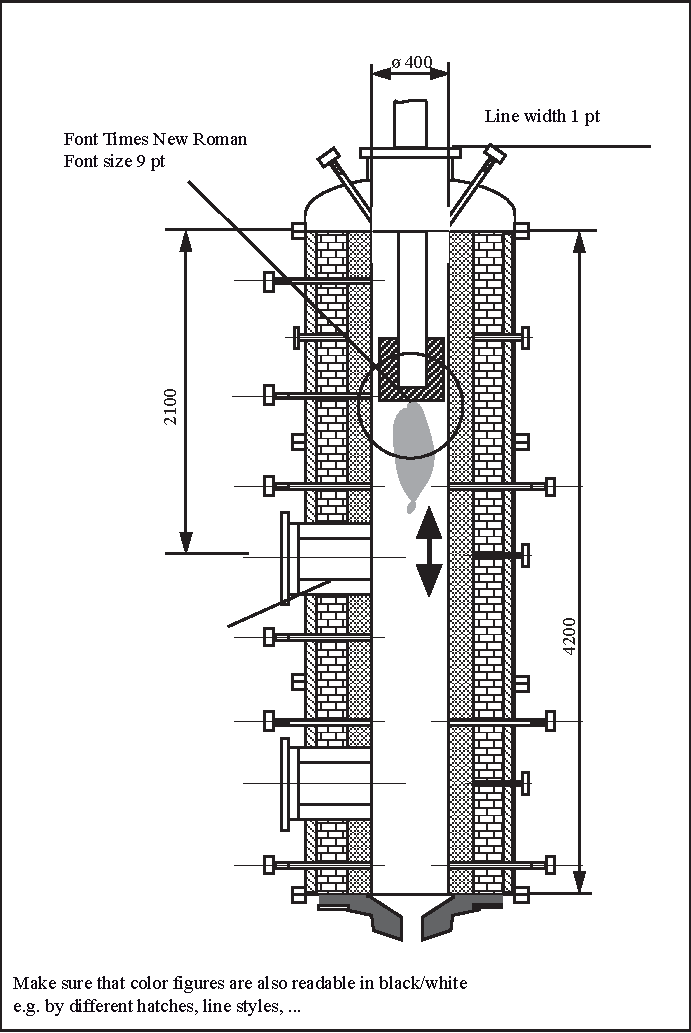
\includegraphics{\ThisPath Figures/Example.pdf}
%	\caption{An example figure to show the dimensions (Max. $117 \times 175$~mm). Please avoid scaling and stick to the instructions provided by Springer.}\label{ex: example figure}
%\end{figure}

Images must be exported/saved as PDF files. Please use vector graphics whenever possible. Please select a maximum width of \SI{11.7}{\centi \meter} and a maximum height of \SI{17.5}{\centi \meter} in the programs you use for this purpose.
Use non-serif font type, font size 10 and a minimum line size of \SI{1}{pt}. Never use the \enquote{scale} command.  

Please save your PDF image files in the subfolder \enquote{Figures}, which is located in your local project folder. Thus, LaTeX can integrate your images into the LaTeX document. For embedding please enter in your tex-file (e.g. C4.tex) in the \enquote{\textbackslash includegraphics} command the file name of your image without the extension ".pdf": \\ 

Labels for images always start with \enquote{fig:}, tables with \enquote{tab:} and equations with \enquote{eq:}. To avoid conflicts with same labeling in other projects use the following structure and reclace only the <individual label> part: \\

\textbackslash label\{fig:\textbackslash Project <individual label>\}



%%%%%%%%%%%%%%%%%%%%%%%%%%%%%%%%%%%%%%%%%%%%%%%
% END OF EXAMPLE
%%%%%%%%%%%%%%%%%%%%%%%%%%%%%%%%%%%%%%%%%%%%%%%
\newpage
\section{Modelling ignition and combustion of solid pulverised fuels under laminar conditions}

\subsection{Combustion of solid fuels with a Resolved-particle approach}
In the resolved particle model, the solid-gas interface and particle boundary layer are resolved chemically and spatially. Simulations based on the resolved particle model can describe interactions between chemistry and transport that can be used to understand the interaction of chemical and transport processes and to develop accurate models for application in large-scale simulations typically using the point particle assumption. A detailed description and validation of the applied resolved particle model is given in Ref.~\cite{Farazi2017}.
%\textcolor{red}{Change here: here, first, you need to write what the resolved approach is and why it is useful.}

\subsubsection{Resolved simulations of single particles}
The combustion of single char particles in a laminar flow field is investigated with spatially and chemically resolved simulations in air and oxy-atmospheres. Mass and energy exchanges between the particle and its surrounding gas are studied and comparisons between the different atmospheres are made. The simulations for the initial comparison are performed for $Re_\mathrm{rel}$ = 1 in both atmospheres. Figure~\ref{fig:B3ResolvedSingleTmax} shows the evolution of the maximum temperature in the gas phase, $T_\mathrm{g,max}$, in both air and oxy-atmospheres. A higher temperature in the oxy- than in the air atmosphere is observed at the early stage of char combustion, while afterwards until $t^{\ast}$ = 60, higher $T_\mathrm{g,max}$ is obtained in the air atmosphere. Moreover, Figure~\ref{fig:B3ResolvedSingle2D} shows that at $t^{\ast}$ = 60, not only $T_\mathrm{g,max}$, but also $T_\mathrm{g}$ around the particle is higher in the air compared to the oxy-atmosphere. The temperatures inside the particle vary almost linearly in time with a heating rate of about $10^{5}$ K/s. The radial changes of temperature inside the particle are less than \SI{10}{K}.
\begin{figure}[h]
	\subfloat[maximum temperature evolution]{\includegraphics[width=0.48\textwidth, height=0.33\textwidth]{\ThisPath Figures/ResolvedApproachSingleParticleCombustion_ValidationModelTmax.pdf}\label{fig:B3ResolvedSingleTmax}}
    \hfill
	\subfloat[2-D distribution of $T_\mathrm{g}$]{\includegraphics[width=0.48\textwidth]{\ThisPath Figures/ResolvedApproachSingleParticleCombustion_ValidationModelAtmosphere.pdf}\label{fig:B3ResolvedSingle2D}}
	\caption{(a) Evolution of the maximum temperature in the gas phase, $T_\mathrm{g,max}$, in both oxy- and air atmospheres with $Re_\mathrm{rel}$ = 1 and $X^{0}_{\ce{O2}}$ = 0.3.\\(b) 2-D distribution of gas phase temperature, $T_\mathrm{g}$, in Kelvin at $t^{\ast}$ = 60.}\label{fig:B3ResolvedSingle}
\end{figure}
%
%Material and energy exchange between the solid particle and the gas phase during combustion in an oxy-fuel atmosphere is investigated and compared with corresponding cases in air ~\cite{Farazi2017}. It is found that the lower carbon consumption rate in oxy-atmosphere results from a higher activity of the reaction \ce{O2} + \ce{H} $\rightarrow$ \ce{OH} + \ce{O}, which consumes \ce{O2} in the gas phase faster leading to a shortage of oxygen for the surface oxidation reaction and consequently to lower heat release due to the lower carbon consumption rate. The combination of a lower heat release and higher specific heat yield lower temperatures in oxy- compared to the air atmosphere.
%\\
%Furthermore, for the typical particle Reynolds numbers and local conditions considered in Ref. ~\cite{Farazi2017}, the convective Damk\"ohler number $Da_\mathrm{conv}$ of the particles is always greater than one, which emphasizes the important role of transport. Therefore, the interaction between transport processes and chemistry is investigated based on a series of simulations with varying particle Reynolds numbers $Re_\mathrm{rel}$.
%\\
%The normalized heat release $\overline{\dot{Q}}/\overline{\dot{Q}}_\mathrm{ref}$ over $Re_\mathrm{rel}$ is shown in Fig. \ref{fig:B3RFCokeCombenA}. In all studied oxy-atmospheres, $\overline{\dot{Q}}/\overline{\dot{Q}}_\mathrm{ref}$ increases with increasing $Re_\mathrm{rel}$ from 0.125 to 4, before it decreases at $Re_\mathrm{rel}$ = 8. As discussed in Ref. ~\cite{Farazi2017}, the heat release from the homogeneous reactions mainly depends on the amount of the oxygen in the atmosphere, the \ce{CO} released due to surface reactions, and the temperature. 
%\\
%Figure \ref{fig:B3RFCokeCombenB} shows for each gas composition that $\overline{\dot{m}}_\mathrm{C}/\overline{\dot{m}}_\mathrm{C,ref}$ first increases with increasing $Re_\mathrm{rel}$ and then decreases at $Re_\mathrm{rel}$ = 2. $\overline{\dot{m}}_\mathrm{C}$ represents the mean CO production rate and is a function of the oxygen concentration and the temperature. It is discussed in detail in Ref. ~\cite{Farazi2017} that increasing $Re_\mathrm{rel}$ enhances the oxygen transport to the combustion zone, while $T_\mathrm{g}$ reduces. Based on these results, it is concluded that from $Re_\mathrm{rel}$ = 0.125 to 2, the higher oxygen concentration compensates the temperature drop and thus $\overline{\dot{m}}_\mathrm{C}/\overline{\dot{m}}_\mathrm{C,ref}$ increases. When $Re_\mathrm{rel}$ increases from 2 to 8, the $Da_\mathrm{conv}$ is low enough to cause a competition between chemistry and transport. This leads to a significant decrease in temperature, and consequently $\overline{\dot{m}}_\mathrm{C}/\overline{\dot{m}}_\mathrm{C,ref}$ decreases. Comparing the $\overline{\dot{m}}_\mathrm{C}/\overline{\dot{m}}_\mathrm{C,ref}$,ref variation over $Re_\mathrm{rel}$ for each gas composition shows that at higher oxygen concentrations, the impact of the flow on the CO production rate is enhanced.
%\begin{figure}
%	\subfloat[Heat release rate]{\includegraphics[width=0.48\textwidth]{\ThisPath Figures/ResolvedApproachSingleParticleCombustion_Q.pdf}\label{fig:B3RFCokeCombenA}}
%    \hfill
%	\subfloat[Coke combustion rate]{\includegraphics[width=0.48\textwidth]{\ThisPath Figures/ResolvedApproachSingleParticleCombustion_m.pdf}\label{fig:B3RFCokeCombenB}}
%	\caption{Heat release rate and coke combustion rate as a function of particle Reynolds number in air and oxy-fuel atmosphere. $\overline{\dot{Q}}_\mathrm{ref}$ and $\overline{\dot{m}}_\mathrm{C,ref}$ correspond to the respective values at $Re_{rel}$ = 1 and $X_\mathrm{O_2}$ = 0.3}\label{fig:B3RFCokeComben}
%\end{figure}


\newpage
\subsubsection{Resolved simulations of particle groups}
An industrial furnace contains millions of burning particles interacting with the surrounding gas flow and their neighbouring particles. Therefore, in addition to the single particle, particle combustion should also be investigated in a group configuration using the particle-resolved approach. To discuss the interaction between the gas flow and the particle group combustion, the particle array configuration from Ref.~\cite{Sayadi2017} is presented here. Similar to the single particle simulations, the particle array configuration has inlet-outlet boundaries in the stream-wise direction. All particles have a diameter of \SI{100}{\micro\metre}, and their initial temperature is the same as the initial gas temperature of \SI{1500}{K}. In this case, the gas phase burns under oxy-fuel conditions~\cite{Sayadi2017}.
\\
A reference case is defined by three particles in a stream-wise direction, with 6$D_\mathrm{p}$ particle spacing and a relative Reynolds number of 1. Figure~\ref{fig:B3RFQandTen} shows the distribution of the heat release rate $\dot{Q}$, temperature $T$, \ce{OH}, and \ce{O2} mass fractions in the vicinity of the particles for the reference case. The first particle (from the left side) upstream behaves similarly to a single particle, while downstream particles behave very differently. All quantities are non-uniformly distributed around particles. The peak of the heat release rate is upstream of the first particle, while the peak of the gas temperature is further downstream. Besides the heat release rate $\dot{Q}$, \ce{OH} and \ce{O2} distributions reveal substantially higher values around the first particle. The non-uniform distribution of the quantities originates from the gas flow, which continuously supplies oxygen for the first particle. The higher \ce{O2} concentration leads to faster oxidation on the surface of the first particle. As a result of the faster surface oxidation rate together with the higher oxygen concentration, the vicinity of the first particle becomes the most active region for exothermic gaseous reactions and yields the highest heat release values.
\begin{figure}[h]
	\includegraphics[width=1.00\textwidth]{\ThisPath Figures/ResolvedApproachParticleGroupCombustion.pdf}
	\caption{Distribution of the heat release rate $\dot{Q}$, temperature $T$, \ce{OH} and oxygen mass fractions in the vicinity of the particles with 6$D_\mathrm{p}$ spacing at $Re_\mathrm{rel}$ = 1. The particles are approached from the left.}\label{fig:B3RFQandTen}
\end{figure}
\\
Further parametric studies, where the particle spacing $L$ is varied from 3$D_\mathrm{p}$ to 9$D_\mathrm{p}$ and the relative Reynolds number $Re_\mathrm{rel}$ from 1 to 8, are discussed and analyzed in Ref. ~\cite{Sayadi2017}.
% last sentence (?) => ask Pooria (should be ok)


\newpage
\subsubsection{Kinetic models for coal and biomass combustion}
The chemical percolation devolatilization (CPD) model describes the devolatilization process of coal based on a detailed description of the molecular structure~\cite{Grant1989}. The CPD coal-dependent input parameters were applied based on the data provided by~\linkproject{A1} and~\linkproject{A2}. Based on this detailed description, the CPD model determines rates for each species released during the devolatilization process and has been shown to accurately represent the devolatilization process of different coals and heating conditions~\cite{Farmand2022}.
% reference to Farmand2022 ok? (Fletcher - Review would be better but an additional reference ...
\\
The mechanistic CRECK-S multi-step devolatilization model ~\cite{Ranzi2008, Debiagi2015} for biomass pyrolysis and gasification was developed in project~\linkproject{A8} and is employed to model the devolatilization process of biomass in this study. The multi-step multi-component kinetics considers 69 species and 39 chemical first-order reactions and treats biomass pyrolysis as a combination of the main biomass constituents: cellulose, hemicellulose, lignin, and extractives. The released species include condensible bio-oils (large polycyclic aromatic hydrocarbons and oxygenates), bio-gas, water, and biochars. A major advantage of this mechanistic model is the predictive capability without tuning stoichiometric for different reference species and activity of rate parameters.
% project or teilproject?
\\\\
Decomposition reactions of the volatile species released during the particle pyrolysis process are modelled with skeletal chemical kinetic models for coal and biomass combustion. The model from Cai et al.~\cite{Cai2021} is used to model coal combustion. An updated version of the detailed chemical kinetic model from Langer et al.~\cite{Langer2023} is used as the base-chemistry model for the development of a skeletal chemical kinetic model for biomass combustion at high temperatures in the partially premixed flame around the particle at atmospheric pressure. The missing anisole (main volatile species for lignin combustion), levoglucosan (cellulose combustion), and propionaldehyde (main volatile around biomass particle ignition) chemistry in the model from Langer et al.~\cite{Langer2023} is extracted from recently published detailed chemical kinetic models~\cite{Wagnon2018, Debiagi2016, Pelucchi2015} and integrated into the base-chemistry model. Using a multi-step reduction strategy involving reaction flux based reduction techniques (DRGEP~\cite{PepiotDesjardins2008} and reaction flux analysis), a skeletal chemical kinetic model for biomass combustion (71 species and 1156 reactions) is obtained and applied in this study. Figure~\ref{fig:B3BioMechValidation} shows model predictions of the developed biomass kinetic model in comparison to respective detailed kinetic models and experimental data under different conditions.
\begin{figure}[h]
    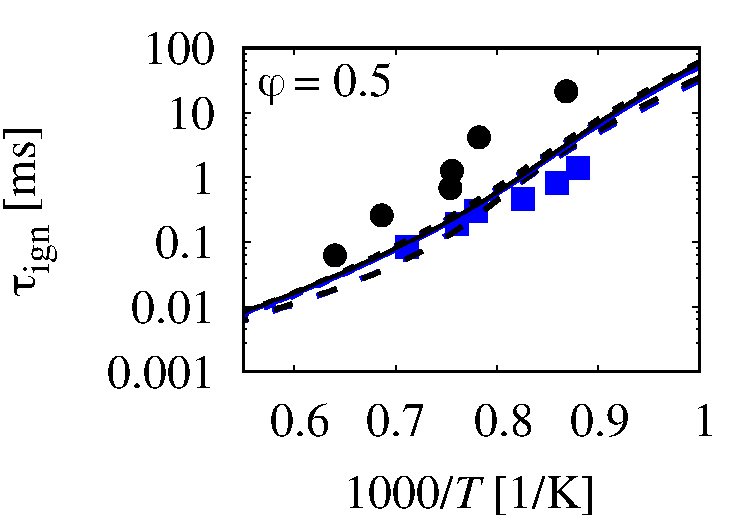
\includegraphics[width=0.32\textwidth]{\ThisPath Figures/IDT_Propanal_Lean.pdf}
    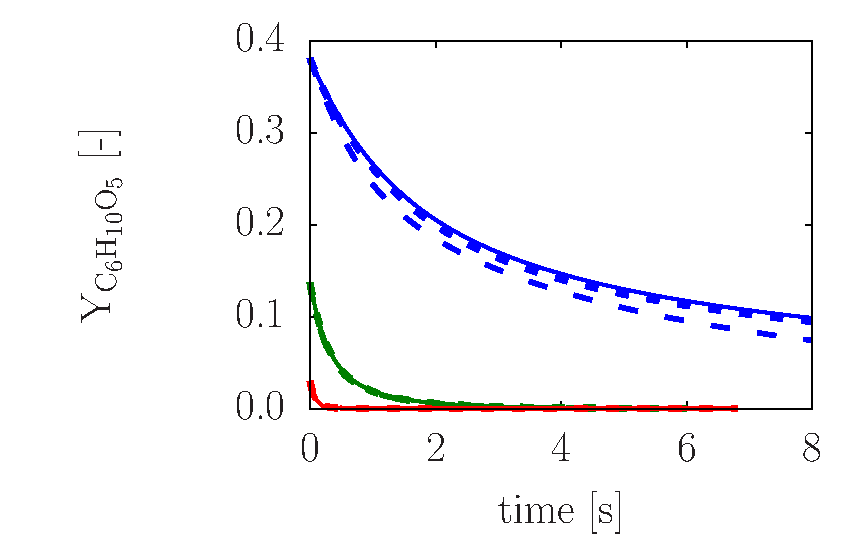
\includegraphics[width=0.32\textwidth]{\ThisPath Figures/CellulosePyrolysis_C6H10O5.pdf}
    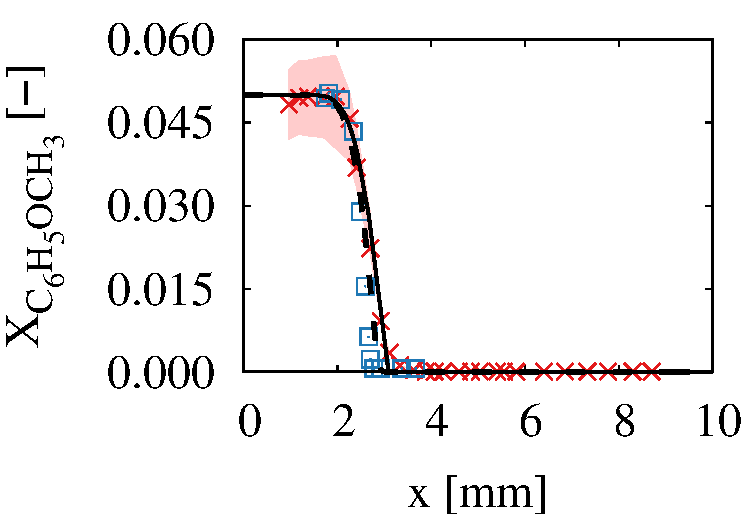
\includegraphics[width=0.32\textwidth]{\ThisPath Figures/Figure_6a.pdf}
    \caption{Comparison of model predictions of the skeletal biomass model (solid lines), the respective detailed kinetic model merged with the base-chemistry model (dotted lines), the detailed reference model (dashed lines), and experimental data (if present)~\cite{Pelucchi2015, Chen2022}.}\label{fig:B3BioMechValidation}
\end{figure}
% ToDo
% oxyfuel conditions mention ???


\newpage
\subsection{NOx Kinetic modelling of solid fuel flames}

\subsubsection{Solid phase modelling}
The release of fuel-bound nitrogen is modelled with the extended nitrogen sub-mechanism of the CRECK-S model~\cite{Debiagi2017} developed in~\linkproject{A8}. Nitrogen characterization and the nitrogen multi-step kinetic sub-mechanism follow the same approach as the hydrocarbon part of the model. Volatile nitrogen containing species released from the solid kinetic model are \ce{NH3}, \ce{HCN}, and \ce{NO}, while tar-N is modelled simplified as pyridine (\ce{C5H5N}) in this study.

\subsubsection{Gas phase modelling}
A chemical kinetic model for NO\textsubscript{x} formation is developed to describe NO\textsubscript{x} formation from the nitrogen containing volatile species released from the CRECK-S model~\cite{Ranzi2008, Debiagi2015}. This chemical kinetic model is based on an ITV-NO\textsubscript{x} model, which is a reduced version of the Glarborg et al. model~\cite{Glarborg2018} and contains an updated ammonia chemistry from the KAUST model~\cite{Zhang2021}. The required pyridine chemistry to model tar-N is adopted from the CRECK-NO\textsubscript{x} model~\cite{Shamooni2021} and integrated into the base-chemistry model. The required NO\textsubscript{x}-chemistry for the application case is extracted from the merged NO\textsubscript{x} formation model based on a reaction flux analysis to obtain a more compact model size. The model predictions of the developed kinetic model are shown in comparison to experimental data in Fig.~\ref{fig:B3NOxMechValidation}.
\begin{figure}[h]
    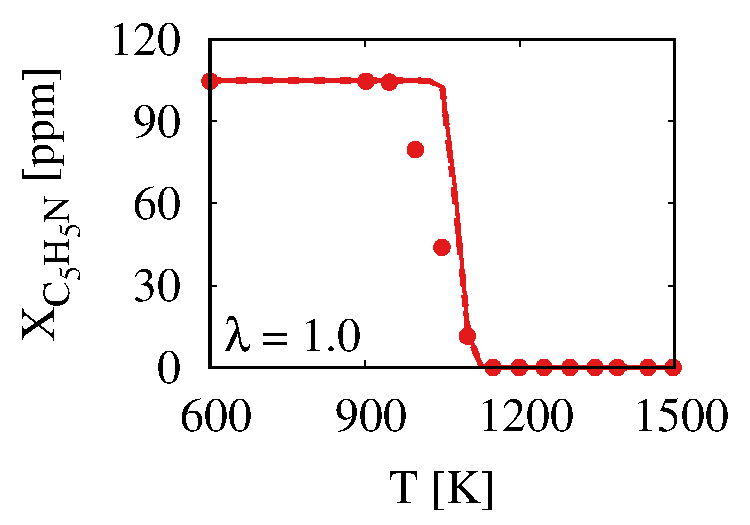
\includegraphics[width=0.32\textwidth]{\ThisPath Figures/Alzueta_C5H5N_Set5.pdf}
    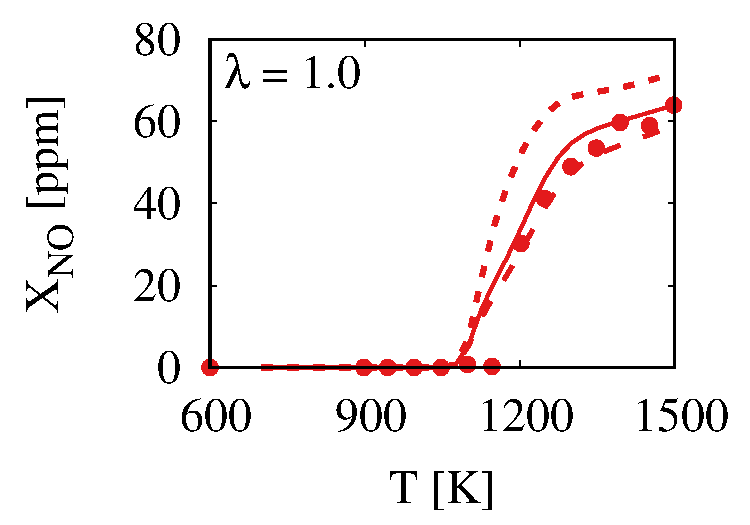
\includegraphics[width=0.32\textwidth]{\ThisPath Figures/Alzueta_NO_Set5.pdf}
    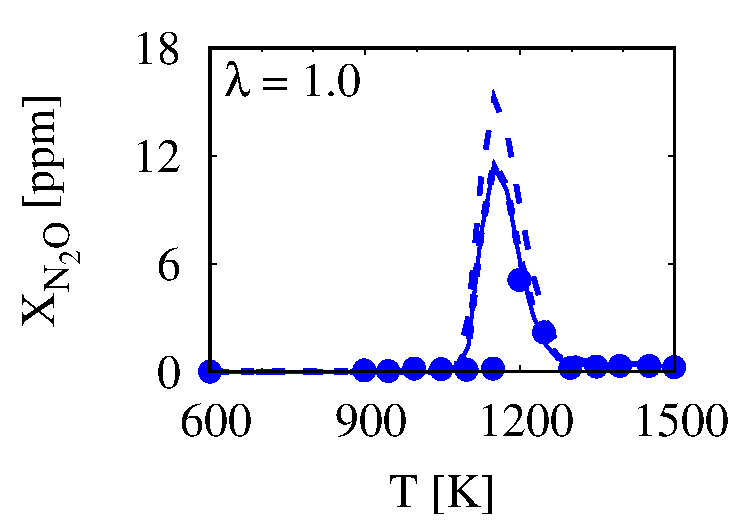
\includegraphics[width=0.32\textwidth]{\ThisPath Figures/Alzueta_N2O_Set5.pdf}
    \caption{Comparison of the model predictions of the developed NO\textsubscript{x} model (solid lines), the full ITV model (dotted lines), the CRECK-NO\textsubscript{x} model~\cite{Shamooni2021} (dashed lines), and the experimental data from Alzueta et al.~\cite{Alzueta2002} (symbols).}\label{fig:B3NOxMechValidation}
\end{figure}
% reference CRECK-S model => algae paper here, or?


%%%%%%%%%
% ToDo
%%%%%%%%%

%%%%%%%%%

%%%%%%%%%%%%%%%%%%%%%%%%%%%%%%%%%%%%%%%%%%%%%%%
% END NEW PART
%%%%%%%%%%%%%%%%%%%%%%%%%%%%%%%%%%%%%%%%%%%%%%%
\newpage
\section{END OF NEW PART}
\clearpage
\section{Resolved approach}
\subsection{Resolved simulations of single particles}
The interactions between the flow field and the combustion of a coal particle were investigated in temporally, spatially, and chemically fully resolved simulations. Particle-resolved simulations are typically conducted for spherical particles. However, microscopic images from TP ~\linkproject{A2} indicate that while this assumption may apply to some particles, others may be better approximated by cylinders, thus both forms should be examined as boundary structures. Initially, infinitely long cylindrical particles were investigated, as these can also be described for particle groups through 2D simulations. Subsequently, simulations for spherical particles were also conducted. For the simulations, an approach similar to that of Lee et al. ~\cite{Lee1996} was used, marking the first time such a transient model for fully resolved simulations of coal combustion in an oxy-fuel atmosphere (\ce{CO2}/\ce{O2} instead of \ce{N2}/\ce{O2}) was employed. The model was implemented in the institute's own simulation code CIAO, described in more detail in Refs. ~\cite{Desjardins2008, Trisjono2016}, and can be used for both devolatilization and coke combustion. The implementation was validated based on the experiments conducted by TP ~\linkproject{A2} on coke combustion in both air and oxy-fuel atmospheres, showing good agreement with the experiments in both environments. Figure ~\ref{fig:B3RFBurnerSetup} illustrates the experimental setup and the calculated temperature distribution for both cases.
\begin{figure}
	\includegraphics[width=1.00\textwidth]{\ThisPath Figures/ModelValidationAndFlatFlameBurner.pdf}
	\caption{Illustration of the model validation. Right side: Flat flame burner from TP A2 with an image of a particle stream during the coke burn-off. Left side: Calculated temperature distribution from the simulation, where the gas temperature $T_\mathrm{g}$ = 1496 K and oxygen content $X_\mathrm{O_2}$ = 0.3}\label{fig:B3RFBurnerSetup}
\end{figure}
\\\\
Furthermore, mass and energy exchange between the solid particle and the gas phase during combustion in an oxy-fuel atmosphere were investigated and compared with corresponding cases in an air atmosphere. For both atmospheres, an energy balance analysis revealed that the majority of heat release occurs not through heterogeneous reactions but through gas-phase reactions involving components released by heterogeneous reactions. Additionally, in an oxy-fuel atmosphere, both a lower coke combustion rate and an overall lower heat release rate compared to combustion in an air atmosphere were observed. Detailed chemical mechanisms were used to analyze the intermediate reactions involved. The lower coke combustion rate in an oxy-fuel atmosphere leads to increased activity of the reaction \ce{O2} + H $\rightarrow$ OH + O, resulting in oxygen deficiency for surface oxidation reactions and consequently lower heat release. The combination of lower heat release and higher specific heat capacity of the gas phase leads to lower temperatures in oxy-fuel compared to air atmospheres.
\\
For the typical particle Reynolds numbers and local conditions considered here, the convective Damk\"ohler number ($Da_\mathrm{konv}$) of the particles is always greater than one, indicating that transport processes play an important role. Therefore, the interaction between transport processes and chemistry was investigated based on a series of simulations with varying particle Reynolds numbers ($Re_\mathrm{rel}$). $Re_\mathrm{rel}$ was modified via the relative velocity U01. Figure ~\ref{fig:B3RFCokeComb} on the left shows a nonlinear trend, where the coke combustion rate increases with increasing Reynolds number until $Re_\mathrm{rel}$ = 2, after which it decreases again. Increasing $Re_\mathrm{rel}$ leads to higher oxygen supply but reduces surface temperature due to increased convection, thus decreasing reaction rates. Above $Re_\mathrm{rel}$ > 2, the reduction in surface temperature predominates, causing the coke combustion rate to decrease. This behavior was also observed under different oxygen concentrations. Figure ~\ref{fig:B3RFCokeComb} also shows that the coke combustion rate in an oxy-fuel atmosphere is always lower than in an air atmosphere for the investigated cases with the same oxygen concentration. The release, as shown in Fig. ~\ref{fig:B3RFCokeComb} on the right, changes with $Re_\mathrm{rel}$ similarly to the coke combustion rate. Heat release through homogeneous gas-phase reactions depends mainly on available oxygen in the atmosphere, coke combustion rate, and temperature. It is further observed that the reduction in temperature and coke combustion rate only surpasses the influence of higher oxygen concentrations on homogeneous reactions at $Re_\mathrm{rel}$ > 4, resulting in an overall decrease in heat release.
\begin{figure}
	\includegraphics[width=1.00\textwidth]{\ThisPath Figures/CokeCombusitonRateAndHeatReleaseRate.pdf}
	\caption{Coke combustion rate and heat release rate as a function of particle Reynolds number in air and oxy-fuel atmosphere. $\overline{\dot{m}}_\mathrm{C,ref}$ and $\overline{\dot{Q}}_\mathrm{ref}$ correspond to the respective values at $Re_{rel}$ = 1 and $X_\mathrm{O_2}$ = 0.3}\label{fig:B3RFCokeComb}
\end{figure}
\\
In the model used here, the influence of porosity was accounted for by a constant effectiveness factor in the rates of heterogeneous reactions. This factor represents the ratio of the surface area available for heterogeneous reactions, including the particle's internal pore structure, to the nominal surface area of the particle without considering the pores. However, this ratio not only depends on the type of solid fuel but also changes with increasing porosity during particle combustion. Sensitivity analyses revealed that the effectiveness factor has a particularly strong influence on combustion behavior. Therefore, in the second funding period, improved models for the influence of porosity will be developed in close collaboration with TP ~\linkproject{A6}.
\\
The data and insights obtained from the simulations described here can further inform model development. This will be presented following the discussion of simulations of particle groups.
% ToDo
% remove "TP"? (see TP A2)

\subsection{Resolved simulations of particle groups}
Particle group combustion was also investigated through fully resolved simulations of various configurations. The parameter space for these simulations includes different gas compositions, particle Reynolds numbers, Damk\"ohler numbers, particle spacing's, particle numbers, and group arrangements, and was conducted for infinitely long cylinders, similar to single particle simulations. The particle spacing L was varied between 3 $D_\mathrm{p}$ and 9 $D_\mathrm{p}$, where $D_\mathrm{p}$ represents the particle diameter. This corresponds to the range resulting from the typical particle number densities calculated by TP ~\linkproject{C2} for the 100 kW swirl burner used in TP ~\linkproject{C1} at Aachen. In most cases, the behavior of the first particle upstream is similar to that of a single particle, while particles downstream exhibit significantly different behavior. A reference case was defined with three horizontally arranged particles, L = 6 $D_\mathrm{p}$, and $Re_\mathrm{rel}$ = 1. Figure ~\ref{fig:B3RFQandT} shows the heat release, temperature, and mass fractions of OH and \ce{O2} in the vicinity of the particles. The surrounding gas phase of the first particle contains significantly more oxygen than the surrounding gas phases of the rear particles, so the highest heat release rate is observed at the first particle despite higher temperatures at the rear particles. With the same particle spacing, the influence of a Reynolds number change depends on the particle position. The coke combustion rate at the first upstream particle shows a maximum similar to that of single particles, after which an increase in the Reynolds number leads to a reduction in the coke combustion rate. However, the coke combustion rate at the second and third particles increases monotonically with $Re_\mathrm{rel}$. At $Re_\mathrm{rel}$ = 8, the third particle shows its highest coke combustion rate due to the increased oxygen concentration and temperature at the surface. Further studies of various parameters have shown that the coke combustion rate of downstream particles increases with increasing Reynolds number regardless of particle spacing and oxygen concentration in the atmosphere. Figure ~\ref{fig:B3RFQandT} also shows that an increase in the Reynolds number enlarges the flame front and leads to a different flame structure. At small particle spacings, an increased Reynolds number leads to particle group combustion, while at larger particle spacings, each particle behaves similarly to a single particle.
\begin{figure}
	\includegraphics[width=1.00\textwidth]{\ThisPath Figures/HeatReleaseRateTemperatureYOHandYO2.pdf}
	\caption{Heat release rate $\dot{Q}$, temperature $T$, OH and \ce{O2} mass fractions near the particle at a particle distance of 6 $D_\mathrm{p}$ and $Re_\mathrm{rel}$ = 1. The particles are approached from the left.}\label{fig:B3RFQandT}
\end{figure}
\begin{figure}
	\includegraphics[width=1.00\textwidth]{\ThisPath Figures/HeatReleaseAndTemperature.pdf}
	\caption{Heat release $\dot{Q}$ and temperature distribution $T$ near the particles for different configurations (particle distances of 3, 6, and 9 $D_\mathrm{p}$) at $Re_\mathrm{rel}$ = 1 and 8.}\label{fig:B3RFQandTandOHandO2}
\end{figure}
\\\\
For all particle spacings, an increase in $Re_\mathrm{rel}$ leads to a shift of the temperature peak towards the outlet. To compare the heat release at different particle spacings while keeping the Reynolds number constant, the volume-averaged heat release was calculated, as shown in Fig. ~\ref{fig:B3RFQandTandOHandO2}. It is evident from this that a denser particle cloud at lower Reynolds numbers results in a decrease in heat release, while dense particle clouds at higher Reynolds numbers lead to particle group combustion and thus significantly higher heat release. The curve for single particles corresponds to the limiting case for infinitely large particle spacings. Further parameter studies were conducted and analyzed to incorporate the results regarding particle interaction into the model development for the point particle approach.
\begin{figure}
	\includegraphics[width=1.00\textwidth]{\ThisPath Figures/VolAverageHeatReleaseAndTemperatureDistribution.pdf}
	\caption{Volume-averaged heat release and temperature for different particle distances and $Re_\mathrm{rel}$. In each case, the gas temperature corresponds $T_\mathrm{g}$ = 1496 K and oxygen mass fraction $Y_\mathrm{O_2}$ = 0.3. $\overline{\dot{Q}}_{ref}$ and $\overline{T}_\mathrm{g,ref}$ correspond to to the respective value at $Re_\mathrm{rel}$ = 1.}\label{fig:B3VolQandT}
\end{figure}




\section{Point particle approach}
% ToDo

\subsection{Methods and models} 
\subsubsection{Solid phase} 
The chemical percolation devolatisation (CPD) model was used to describe the devolatilization process ~\cite{Grant1989} of coal. The CPD coal-dependent input parameters were applied based on the data provided by ~\linkproject{A1} and ~\linkproject{A2}. The CPD model has been shown to represent the devolatilization process of different coals and heating conditions with good accuracy. However, its use in computational fluid dynamics is limited because of its relatively high computational cost. While the full CPD model was used in the simulations for this project, an artificial neural network (ANN) based CPD model for predicting coal devolatilization kinetics was developed in collaboration with Zhejiang University in China during a six-month visit of Dr. Yun Bai at ITV in 2017 ~\cite{Xing2019}. The model is based on a database constructed with the CPD model for a wide range of coals and heating rates. The heating rates and the information of ultimate and proximate analysis were chosen as inputs of the ANN model to consider the effects of coal types and heating conditions on coal devolatilization. The outputs are the coal- and operation-specific parameters for a two-step kinetic model. The learning, validation, and application results show that the proposed ANN model has a competitive prediction capability on both the total volatile release and release rates when compared with the CPD model, but has obvious computational efficiency advantages.
% see FP3
\\
The mechanistic CRECK-S-B multistep devolatilization model ~\cite{Ranzi2008, Debiagi2015} for biomass pyrolysis and gasification is used to model the devolatilization process of biomass particles in this study. The multistep multicomponent kinetics considers 69 species and 39 chemical first-order reactions and treats biomass pyrolysis as a combination of the main biomass constituents: cellulose, hemicellulose, lignin, and extractives. The released species include condensible bio-oils (large polycyclic aromatic hydrocarbons and oxygenates), bio-gas, water, and biochars. A major advantage of this mechanistic model is the predictive capability without tuning stoichiometric for different reference species and activity of rate parameters.


\subsubsection{Gas phase} 
Decomposition reactions of the volatile species released during the particle pyrolysis process are modelled with skeletal chemical kinetic models for coal and biomass combustion. An updated version of the detailed chemical kinetic model from Langer et al. ~\cite{Langer2023} is used as the base-chemistry model for the development of skeletal chemical kinetic models for coal and biomass combustion at high temperatures in the partially premixed flame around the particle at atmospheric pressure. The missing anisole (main volatile species for coal and lignin combustion), levoglucosan (cellulose combustion), and propionaldehyde (main volatile around biomass particle ignition) chemistry in the model from Langer et al. ~\cite{Langer2023} is extracted from recently published detailed chemical kinetic models ~\cite{Wagnon2018, Debiagi2016, Pelucchi2015} and integrated into the base chemistry model. Based on a multi-step reduction strategy involving reaction flux based reduction techniques (DRGEP ~\cite{PepiotDesjardins2008} and reaction flux analysis), skeletal chemical kinetic models for coal (56 species and 838 reactions) and biomass (71 species and 1156 reactions) are obtained and applied in this study.
% ToDo
% coal mechanism here ???
% validation figures(s) (?)
% oxyfuel conditions => validation => some figures (otherwise no reference...)


\subsubsection{Interphase coupling} 
The two-phase interaction between the solid particle and the gas phase was modelled using an Euler-Lagrange approach. In this approach, gas-phase equations are solved in the Eulerian framework, while particle equations are written in the Lagrangian framework. The Euler and the Lagrange equations are fully coupled using a two-way coupling approach. The models are described in detail by Farazi et al. ~\cite{Farazi2019a, Farazi2019b}. The models were implemented in the in-house simulation code CIAO ~\cite{Trisjono2016} and are applicable for various pulverised fuels. For the Euler-Lagrange approach, particle equations were derived according to the film model. As described by Farazi et al. ~\cite{Farazi2017b}, the film model was used to describe the coupling of the continuous and the dispersed phase. In the context of the point-particle methods, the ratio of cell size to particle size is critical. The derivation of the film relies on the assumption of a homogeneous far-field around the particles, which in turn necessitates large cell to particle size ratios. However, using large cell sizes, gas-phase ignition cannot fully be captured due to diluted mixtures, as shown by a convergence study in Farazi et al. ~\cite{Farazi2019a, Farazi2019b}. Therefore, a new numerical formulation was developed that allows the computational cell size to be of the same order as the particle diameter, which requires the consideration of two aspects. First, the resulting already mentioned inconsistencies in the film model assumptions need to be addressed. Second, for relatively small cells, large source terms appear in the continuous phase from the mass and heat release of particles. These may lead to numerical instabilities. To overcome the first challenge, a filtering method is developed to provide smoother gas-phase fields as input for the Lagrange phase leading to a more consistent evaluation of the state of the particle surroundings ~\cite{Farazi2019b}. The large particle source terms in the gas phase are numerically tackled by introducing a distribution function of the Eulerian source term to multiple cells based on a Gaussian kernel function ~\cite{Farazi2019b}. This numerical method has been provided to ~\linkproject{C2} to improve the Euler-Lagrange description in the overall OxySim-129 simulation framework ~\cite{Nicolai2021}.
% see FP3 


\subsection{Modeling ignition and combustion of coal and biomass in laminar configuration} 
\subsubsection{Single-particle combustion}
Since modelling ignition and combustion of coal particles requires a significant number of physical models and simplifying assumptions, a validation of ignition delay times of a single-particle with available experimental measurements and comparison with previously published numerical results were performed, as shown in Fig. ~\ref{fig:B3SingleValidation} a) and ~\ref{fig:B3SingleValidation} b) ~\cite{Attili2020, Farazi2019a}. The comparison with the experiments from ~\linkproject{B7}, shown in Fig. ~\ref{fig:B3SingleValidation} c) also shows good agreement with measured ignition delay times for variations in particle diameter $D_\mathrm{p}$ ~\cite{Attili2020, Li2021}.
\begin{figure}
	\includegraphics[width=1.00\textwidth]{\ThisPath Figures/Validation_new.pdf}
	\caption{a) Ignition times for various particle diameters compared with experimental data reported by Liu et al. ~\cite{Liu2011} and numerical data by Goshayeshi and Sutherland ~\cite{Goshayeshi2014}\\b) Ignition delay times for various initial gas temperatures compared with experimental data reported by Liu et al. ~\cite{Liu2011} and numerical data by Goshayeshi and Sutherland ~\cite{Goshayeshi2014}\\c) Ignition delay times for various particle diameters compared with B7 experimental data ~\cite{Attili2020}}\label{fig:B3SingleValidation}
\end{figure}
These results were analysed in more detail. The ignition of coal particles and the volatile flame surrounding a particle were found to be strongly influenced by the release rate of volatiles. In particular, the volatiles release rate was observed to possess a double peak behaviour in time. The ignition can happen during the onset of the first or second peak, depending on the particle size and boundary conditions ~\cite{Farazi2019a}. Generally, an earlier onset of ignition was observed for higher initial gas temperatures and smaller particles, which heat-up faster than large particles due to their lower thermal inertia. It was also observed that ignition in mixtures with significant amounts of \ce{CO2} diluent is slower compared with the cases in air atmosphere. As shown in Fig. ~\ref{fig:B3SingleAirOxy} a), it was found that this difference is more significant for lower initial gas temperatures. A reaction pathway analysis reveals that in an oxy-fuel atmosphere, the rate of reaction \ce{CO2} + H $\rightarrow$ CO + OH is higher compared with that in air atmosphere due to the higher \ce{CO2} concentrations. Since the high concentration of \ce{CO2} causes a strong depletion of H radicals (cf. Fig. ~\ref{fig:B3SingleAirOxy} b)), the production of radicals is decelerated. Consequently, the reactivity of the mixture is reduced, which results in delayed ignition ~\cite{Farazi2019a}.
\\\\
Another important aspect of the coal combustion process is the change of the particles internal structure during different combustion stages. In FP1, a significant influence of the particle porosity on the coal conversion rate was observed in the char combustion investigation using a particle-resolved approach, where porosity was not computed but appeared as an estimated parameter. Despite this importance, the char particles initial porosities are typically unknown. Therefore, in FP2, the particle porosity during the devolatilization phase was computed based on the particle density and mass to provide insight into the char particles initial porosity. Figure ~\ref{fig:B3SinglePorosity} shows the particle porosity evolution in both air and oxy-fuel atmospheres at different initial gas temperatures and various particle diameters. The release of volatiles accelerates pore formation and thus particle porosity evolution. In each atmosphere, smaller particles experience a faster increase in porosity. Comparing the cases with air and oxy-fuel atmospheres, the porosity of the bigger particles is found to evolve slower in the oxy-fuel atmosphere. As Fig. ~\ref{fig:B3SinglePorosity} shows, increasing initial gas temperatures accelerates the particle porosity evolution due to the faster devolatilization process. At the end of the devolatilization process, the particle porosities reach a certain value, which is then considered as the initial porosity for the char conversion. This value depends on the volatile content, the coal type, and the density of the particle.
\begin{figure}
	\includegraphics[width=1.00\textwidth]{\ThisPath Figures/AirOxy_new.pdf}
	\caption{a) Ignition delay times for various particle diameters and gas-phase temperatures in air and oxy-fuel atmospheres\\b) Evolution of maximum H and OH radical mass fractions for \SI{125}{\micro\metre} particles in air and oxy-fuel atmospheres with initial temperature of $T_\mathrm{g}$ = 1200 K}\label{fig:B3SingleAirOxy}
\end{figure}
\begin{figure}
	\includegraphics[width=1.00\textwidth]{\ThisPath Figures/porosity_new.pdf}
	\caption{a) Evolution of the particle porosity for different particle diameters $D_\mathrm{p}$ in oxy-fuel atmosphere at different initial gas temperatures\\b) Evolution of the particle porosity for air and oxy-fuel atmospheres with the same initial gas temperature}\label{fig:B3SinglePorosity}
\end{figure}
% ToDo
% only coal => biomass is missing!


\subsubsection{Particle group combustion}
In addition to the study of single particles, the ignition process of particle streams in air and oxy-fuel atmospheres was simulated. To investigate the effect of interacting volatile flames, two different configurations were studied. The first configuration is a 3D channel with inlet and outlet boundaries in the streamwise direction, while periodicity is imposed in the two span-wise directions. For the channel configuration, coal particles were seeded directly into a hot oxidiser stream. This configuration is representative of a typical industrial burner, where the mixing time is faster than the particle heating time.
\\
After injection, $T_\mathrm{g}$ drops in the vicinity of the particles because of particle heating. Figure ~\ref{fig:B3GroupParticle} a) shows the evolution of particle temperature $T_\mathrm{p}$ and gas temperature $T_\mathrm{g}$ for the particle streams and the single-particle case. As particles move forward, their temperatures gradually increase by energy transfer from the gas phase. After approaching sufficiently high temperatures, the release of volatile gases begins. Moving further downstream, at a certain distance from the inlet for each case, volatile ignition happens indicated by a rapid increase in the gas temperature $T_\mathrm{g}$.
\\
The ignition delay times were determined after reaching a statistically steady-state by means of the ignition position and the averaged particle velocity for different cases of varying particle number density, gas temperature, and injection velocity. As Fig. ~\ref{fig:B3GroupParticle} b) shows, increasing particle number density shifts the ignition location downstream and increases the ignition delay time because of the increased amount of thermal energy needed for particle heating. Increasing the particle number density also affects the volatile flame shape, devolatilization rate, velocity profile, and particle distribution. Figure ~\ref{fig:B3GroupParticle} b) shows two different flame shapes and corresponding ignition distances for the particle streams with different particle number densities. A continuous flame region (group combustion) instead of the spherical diffusion flame around individual particles was observed at a higher number of particles ~\cite{Farazi2019b}.
\\
For this channel configuration, particles were injected over the entire cross-section of the channel inlet. The significant cooling effect observed in this quasi-homogeneous case represents a simplified limiting case. Therefore, a particle jet in a hot co-flow, based on the ~\linkproject{B7} laminar flat flame burner experiment, was investigated as a second case, where the thermal effect is limited due to a smaller number of particles. Moreover, the study was conducted in close collaboration with ~\linkproject{C2} to assess different modelling assumptions for devolatilization, ignition, and combustion. As shown in Fig. ~\ref{fig:B3TurbulenceValidation} a), the ~\linkproject{B3} detailed model simulations (finite rate chemistry CPD (FC-CPD)) for both gas and solid phases were successfully validated with ignition delay times experimentally measured by ~\linkproject{B7}.
\begin{figure}
	\includegraphics[width=1.00\textwidth]{\ThisPath Figures/particle_tm_new.pdf}
	\caption{a) Distribution of average gas temperatures $\left\langle\tilde{T}_{\mathrm{g}}\right\rangle$, and average particle temperatures $\left\langle\tilde{T}_{\mathrm{p}}\right\rangle$, of streams with different particle number densities together with the single-particle case: For each case, the ignition location point is marked with a vertical line.\\b) Distribution of gas temperature $T_\mathrm{g}$, heat release rate $\dot{Q}_\mathrm{g}$, and the mass fraction of \ce{O2} on the x-y plane}\label{fig:B3GroupParticle}
\end{figure}
\\
The validated detailed simulations allow an in-depth analysis of the physical processes occurring during the transition from single-particle to particle group combustion at different particle injection rates. This transition can be observed in the different flame shapes shown in Fig. ~\ref{fig:B3TurbulenceValidation} b). It was found that for low particle injection rates, the volatiles mainly burn in diffusion flames formed around individual particles similar to the single-particle behaviour studied by Farazi et al. ~\cite{Farazi2019a}. By increasing the injection rate, due to oxygen deficiency and relatively lower gas temperatures around the centreline, a delay in the ignition and a more continuous flame region around the particle clouds were observed. This behaviour was found to be more pronounced for higher particle injection rates, in which the flame is suppressed in the centre and consequently limited to the area in the boundary region, where the ignitable mixtures are formed due to the mixing of volatiles with the oxidiser.
\\
In addition to the investigation of physical processes, the complete thermo-chemical state can be extracted from the ~\linkproject{B3} detailed simulations, which allows for the detailed assessment of the reduced-order models used in ~\linkproject{C2} for particle group combustion and a comprehensive investigation of each reduction step to evaluate the assumptions involved in pulverised fuel flamelet generated manifold (FGM) modelling. As shown in Fig. ~\ref{fig:B3TurbulenceValidation} a), using FGM modelling coupled with simplified devolatilization models leads to underpredicted ignition times. The reason for this was analysed jointly with ~\linkproject{C2} by a systematic model simplification approach. The ~\linkproject{B3} simulation framework uses the CPD model for devolatilization, where the volatile composition changes in time ~\cite{Farazi2019a}. In contrast, the current FGM formulation is limited to use one fixed volatile composition to create the flamelet tables. It was found that using this simplifying assumption leads to a shift in the release of different volatiles. However, it has a minor effect on particle group ignition, which shows the validity of this assumption for this case. In contrast, it was found that tabulated chemistry has deficits, especially in the central region, where the fuel-rich mixture exceeds the flammability limits and extrapolation in the table is used. It was also found that simplified yet well-fitted devolatilization models can also predict ignition reasonably well compared to detailed devolatilization models. However, as the parameters are quite sensitive to the heating rate, the quantitative agreement is very dependent on the heating rates used for fitting the parameters. Detailed analyses are presented in Farmand et al. ~\cite{Farmand2022}.
\begin{figure}
	\includegraphics[width=1.00\textwidth]{\ThisPath Figures/jet_validation_new3.pdf}
	\caption{a) Comparison of computed ignition delay times of B3 detailed simulations (FC-CPD) with B7 experiments and C2 FGM model for different injection rates. the error bars correspond to different thresholds of $Y_\mathrm{OH}$.\\b) Instantaneous field of OH mass fraction at steady-state conditions showing different flame shapes in the co-flow jet configuration, which is the effect of different particle injection rates.}\label{fig:B3TurbulenceValidation}
\end{figure}
% ToDo
% only coal => biomass is missing!



\subsection{Modeling ignition and combustion in turbulent conditions} 
% see FP3 (Pulverised coal combustion in homogeneous isotropic turbulence)
The analyses of single-particle and particle group ignition in laminar conditions showed that slip velocity has a significant impact on ignition ~\cite{Attili2020, Farazi2019b, Li2021}. When particles are exposed to turbulent conditions, they face different slip velocities due to the fluctuations in a turbulent flow. To understand the effects of velocity fluctuations in turbulence on ignition and combustion of particle groups, an isotropic turbulent box configuration with periodic boundary conditions in all directions was selected, as shown in Fig. ~\ref{fig:B3TurbulenceBox}.
\\
The first step in studying turbulent coal combustion is to investigate ignition and combustion in the selected configuration for individual, non-interacting particles, as shown in Fig. ~\ref{fig:B3TurbulenceBox} a). It was found that exposure to isotropic turbulent conditions leads to faster ignition compared with laminar conditions. Two important observations were made from the DNS results. First, it was found that the main affecting parameter in isotropic turbulence is the turbulent kinetic energy, which at fixed Reynolds number has a much stronger influence than the integral length scale. Consequently, computing the laminar case with a slip velocity calculated by the average value in the isotropic turbulence case leads to the same ignition delay time. Hence, turbulence effects on ignition are similar to the slip velocity effects in laminar conditions described by Attili et al. ~\cite{Attili2020}. Second, solid fuel particles have a much higher density than the surrounding gas. Hence, they have large Stokes numbers and do not fully follow the flow. This behaviour leads to particle clustering in turbulent flows. As Fig. ~\ref{fig:B3TurbulenceBox} b) shows, for combustion of particle groups in isotropic turbulence, particle clusters form leaving behind regions almost void of particles, where ignition preferentially happens. After ignition, the flame spreads similarly to the laminar channel configuration through the entire domain by igniting other clusters until all of the particles ignited and a continuous flame has established.
\begin{figure}
	\includegraphics[width=1.00\textwidth]{\ThisPath Figures/turbulent_box_new.pdf}
	\caption{Ignition of coal particles in isotropic turbulence:\\a) Individual, non-interacting particles b) High particle number density, where different ignition kernels are observed in regions of lower local particle number densities. Particle temperatures are the same at ignition time due to uniform heating before the ignition. Ignition kernels are shown using the isosurface for 10 \% of $Y_\mathrm{OH,max}$ coloured with the heat release rate $\dot{Q}_\mathrm{g}$ (dark blue shades). Light blue shades represent the velocity isosurface at 30 m/s.}\label{fig:B3TurbulenceBox}
\end{figure}
\\
To evaluate the impact of the particle shape for future investigations of biomass combustion, the particle dynamics of ellipsoidal particles in isotropic turbulence were studied together with ~\linkproject{B2} based on the novel correlations derived in ~\cite{Frhlich2020}. It was shown in a recently submitted manuscript ~\cite{Frhlich2021} that the correlations have a massive impact on the particle dynamics for particle aspect ratios relevant for biomass particles.


\subsection{Modeling pollutant formation in coal and biomass} 

\subsubsection{Chemical kinetic model for NO\textsubscript{x} formation}
A chemical kinetic model for NO\textsubscript{x} formation is used which was developed to describe NO\textsubscript{x} formation from the nitrogen containing volatile species released from the CRECK-S model \cite{Ranzi2008, Debiagi2015}. This chemical kinetic model is based on an ITV-NO\textsubscript{x} model, which is a reduced version of the Glarborg et al. model ~\cite{Glarborg2018} with an updated ammonia chemistry from the KAUST model ~\cite{Zhang2021}. The required pyridine chemistry to model tar-N was adapted from the CRECK-NO\textsubscript{x} model ~\cite{Shamooni2021} and integrated into the base-chemistry model. The merged modular NO\textsubscript{x} formation model contains two modified reaction rates for the NCO chemistry due to an overpredicted NO formation and was extracted to obtain a more compact model size. 
% ToDo
% validation figures required ???

 
\section{Conclusion} 


%%%%%%%%%%%%%%%%%%%%%%%%%%%%%%%%%%%%%%%%%%
% NOTES - Christian
%%%%%%%%%%%%%%%%%%%%%%%%%%%%%%%%%%%%%%%%%%
% Literature only in literature in .bib file => necessary to upload the pdf file (?!)
%%%%%%%%%%%%%%%%%%%%%%%%%%%%%%%%%%%%%%%%%%


%%%% DON'T CHANGE ANYTHING FROM HERE UNTIL NEXT MARKER!
\Acknowledgement

%\ThisPath 
\renewcommand{\bibname}{References}
\begin{btSect}{\ThisPath  Literature/Literature}
	\btPrintCited
\end{btSect}

\end{btUnit}
%%%% DONT CHANGE ANYTHING UNTIL HERE!
